% Options for packages loaded elsewhere
\PassOptionsToPackage{unicode}{hyperref}
\PassOptionsToPackage{hyphens}{url}
%
\documentclass[
]{article}
\usepackage{amsmath,amssymb}
\usepackage{lmodern}
\usepackage{iftex}
\ifPDFTeX
  \usepackage[T1]{fontenc}
  \usepackage[utf8]{inputenc}
  \usepackage{textcomp} % provide euro and other symbols
\else % if luatex or xetex
  \usepackage{unicode-math}
  \defaultfontfeatures{Scale=MatchLowercase}
  \defaultfontfeatures[\rmfamily]{Ligatures=TeX,Scale=1}
\fi
% Use upquote if available, for straight quotes in verbatim environments
\IfFileExists{upquote.sty}{\usepackage{upquote}}{}
\IfFileExists{microtype.sty}{% use microtype if available
  \usepackage[]{microtype}
  \UseMicrotypeSet[protrusion]{basicmath} % disable protrusion for tt fonts
}{}
\makeatletter
\@ifundefined{KOMAClassName}{% if non-KOMA class
  \IfFileExists{parskip.sty}{%
    \usepackage{parskip}
  }{% else
    \setlength{\parindent}{0pt}
    \setlength{\parskip}{6pt plus 2pt minus 1pt}}
}{% if KOMA class
  \KOMAoptions{parskip=half}}
\makeatother
\usepackage{xcolor}
\usepackage[margin=1in]{geometry}
\usepackage{color}
\usepackage{fancyvrb}
\newcommand{\VerbBar}{|}
\newcommand{\VERB}{\Verb[commandchars=\\\{\}]}
\DefineVerbatimEnvironment{Highlighting}{Verbatim}{commandchars=\\\{\}}
% Add ',fontsize=\small' for more characters per line
\usepackage{framed}
\definecolor{shadecolor}{RGB}{248,248,248}
\newenvironment{Shaded}{\begin{snugshade}}{\end{snugshade}}
\newcommand{\AlertTok}[1]{\textcolor[rgb]{0.94,0.16,0.16}{#1}}
\newcommand{\AnnotationTok}[1]{\textcolor[rgb]{0.56,0.35,0.01}{\textbf{\textit{#1}}}}
\newcommand{\AttributeTok}[1]{\textcolor[rgb]{0.77,0.63,0.00}{#1}}
\newcommand{\BaseNTok}[1]{\textcolor[rgb]{0.00,0.00,0.81}{#1}}
\newcommand{\BuiltInTok}[1]{#1}
\newcommand{\CharTok}[1]{\textcolor[rgb]{0.31,0.60,0.02}{#1}}
\newcommand{\CommentTok}[1]{\textcolor[rgb]{0.56,0.35,0.01}{\textit{#1}}}
\newcommand{\CommentVarTok}[1]{\textcolor[rgb]{0.56,0.35,0.01}{\textbf{\textit{#1}}}}
\newcommand{\ConstantTok}[1]{\textcolor[rgb]{0.00,0.00,0.00}{#1}}
\newcommand{\ControlFlowTok}[1]{\textcolor[rgb]{0.13,0.29,0.53}{\textbf{#1}}}
\newcommand{\DataTypeTok}[1]{\textcolor[rgb]{0.13,0.29,0.53}{#1}}
\newcommand{\DecValTok}[1]{\textcolor[rgb]{0.00,0.00,0.81}{#1}}
\newcommand{\DocumentationTok}[1]{\textcolor[rgb]{0.56,0.35,0.01}{\textbf{\textit{#1}}}}
\newcommand{\ErrorTok}[1]{\textcolor[rgb]{0.64,0.00,0.00}{\textbf{#1}}}
\newcommand{\ExtensionTok}[1]{#1}
\newcommand{\FloatTok}[1]{\textcolor[rgb]{0.00,0.00,0.81}{#1}}
\newcommand{\FunctionTok}[1]{\textcolor[rgb]{0.00,0.00,0.00}{#1}}
\newcommand{\ImportTok}[1]{#1}
\newcommand{\InformationTok}[1]{\textcolor[rgb]{0.56,0.35,0.01}{\textbf{\textit{#1}}}}
\newcommand{\KeywordTok}[1]{\textcolor[rgb]{0.13,0.29,0.53}{\textbf{#1}}}
\newcommand{\NormalTok}[1]{#1}
\newcommand{\OperatorTok}[1]{\textcolor[rgb]{0.81,0.36,0.00}{\textbf{#1}}}
\newcommand{\OtherTok}[1]{\textcolor[rgb]{0.56,0.35,0.01}{#1}}
\newcommand{\PreprocessorTok}[1]{\textcolor[rgb]{0.56,0.35,0.01}{\textit{#1}}}
\newcommand{\RegionMarkerTok}[1]{#1}
\newcommand{\SpecialCharTok}[1]{\textcolor[rgb]{0.00,0.00,0.00}{#1}}
\newcommand{\SpecialStringTok}[1]{\textcolor[rgb]{0.31,0.60,0.02}{#1}}
\newcommand{\StringTok}[1]{\textcolor[rgb]{0.31,0.60,0.02}{#1}}
\newcommand{\VariableTok}[1]{\textcolor[rgb]{0.00,0.00,0.00}{#1}}
\newcommand{\VerbatimStringTok}[1]{\textcolor[rgb]{0.31,0.60,0.02}{#1}}
\newcommand{\WarningTok}[1]{\textcolor[rgb]{0.56,0.35,0.01}{\textbf{\textit{#1}}}}
\usepackage{graphicx}
\makeatletter
\def\maxwidth{\ifdim\Gin@nat@width>\linewidth\linewidth\else\Gin@nat@width\fi}
\def\maxheight{\ifdim\Gin@nat@height>\textheight\textheight\else\Gin@nat@height\fi}
\makeatother
% Scale images if necessary, so that they will not overflow the page
% margins by default, and it is still possible to overwrite the defaults
% using explicit options in \includegraphics[width, height, ...]{}
\setkeys{Gin}{width=\maxwidth,height=\maxheight,keepaspectratio}
% Set default figure placement to htbp
\makeatletter
\def\fps@figure{htbp}
\makeatother
\setlength{\emergencystretch}{3em} % prevent overfull lines
\providecommand{\tightlist}{%
  \setlength{\itemsep}{0pt}\setlength{\parskip}{0pt}}
\setcounter{secnumdepth}{5}
\ifLuaTeX
  \usepackage{selnolig}  % disable illegal ligatures
\fi
\IfFileExists{bookmark.sty}{\usepackage{bookmark}}{\usepackage{hyperref}}
\IfFileExists{xurl.sty}{\usepackage{xurl}}{} % add URL line breaks if available
\urlstyle{same} % disable monospaced font for URLs
\hypersetup{
  pdftitle={HUDM6122 Homework\_06},
  pdfauthor={Chenguang Pan},
  hidelinks,
  pdfcreator={LaTeX via pandoc}}

\title{HUDM6122 Homework\_06}
\author{Chenguang Pan}
\date{2023-03-27}

\begin{document}
\maketitle

\hypertarget{github-address}{%
\subsection{Github Address}\label{github-address}}

All my latest homework can be found on Github:
\url{https://github.com/cgpan/hudm6122_homeworks} . Thanks for checking
if interested.

\hypertarget{ex-6.1}{%
\subsection{Ex 6.1}\label{ex-6.1}}

\emph{Apply k-means to the crime rate data after standardising each
variable by its standard deviation. Compare the results with those given
in the text found by standardising by a variable's range.}

\textbf{MY SOLUTION:}

I began this assignment at Mar 27th, at that time there was no
\texttt{crime} dataset available. Therfore, for this homework, I first
extracted the data information from the \texttt{MVA} package and created
the dataset in a csv format for reading convenience. For space-saving
concern, the \texttt{R} syntax to create dataset was in a separated file
called ``HW06\_test.R'', which can be found it in my Github repo.

As discussed on page.179 of the textbook, one need to remove the outlier
(i.e., DC) first.

\begin{Shaded}
\begin{Highlighting}[]
\SpecialCharTok{\textgreater{}} \CommentTok{\# import the dataset}
\ErrorTok{\textgreater{}}\NormalTok{ crime }\OtherTok{\textless{}{-}} \FunctionTok{read.csv}\NormalTok{(}\StringTok{"crime.csv"}\NormalTok{,}\AttributeTok{row.names =} \DecValTok{1}\NormalTok{)}
\SpecialCharTok{\textgreater{}} \FunctionTok{dim}\NormalTok{(crime)}
\NormalTok{[}\DecValTok{1}\NormalTok{] }\DecValTok{51}  \DecValTok{7}
\SpecialCharTok{\textgreater{}} 
\ErrorTok{\textgreater{}} \CommentTok{\# drop the outlier DC and check the dimension of the datset}
\ErrorTok{\textgreater{}}\NormalTok{ df }\OtherTok{\textless{}{-}}\NormalTok{ crime[}\SpecialCharTok{{-}}\FunctionTok{which}\NormalTok{(}\FunctionTok{row.names}\NormalTok{(crime) }\SpecialCharTok{==} \StringTok{"DC"}\NormalTok{),]}
\SpecialCharTok{\textgreater{}} \FunctionTok{dim}\NormalTok{(df)}
\NormalTok{[}\DecValTok{1}\NormalTok{] }\DecValTok{50}  \DecValTok{7}
\SpecialCharTok{\textgreater{}} 
\ErrorTok{\textgreater{}} \CommentTok{\# standardized the variable by its SD}
\ErrorTok{\textgreater{}}\NormalTok{ df\_s }\OtherTok{\textless{}{-}} \FunctionTok{sweep}\NormalTok{(df,}\DecValTok{2}\NormalTok{,}\FunctionTok{apply}\NormalTok{(df, }\DecValTok{2}\NormalTok{, sd), }\AttributeTok{FUN =} \StringTok{"/"}\NormalTok{)}
\SpecialCharTok{\textgreater{}} \FunctionTok{sapply}\NormalTok{(df\_s, var)}
\NormalTok{  Murder     Rape  Robbery  Assault Burglary    Theft  Vehicle }
       \DecValTok{1}        \DecValTok{1}        \DecValTok{1}        \DecValTok{1}        \DecValTok{1}        \DecValTok{1}        \DecValTok{1} 
\SpecialCharTok{\textgreater{}} 
\ErrorTok{\textgreater{}} \CommentTok{\# similar to textbook, I use the within group variance to }
\ErrorTok{\textgreater{}} \CommentTok{\# investigate the appropriate number of cluster}
\ErrorTok{\textgreater{}}\NormalTok{ n }\OtherTok{\textless{}{-}} \FunctionTok{nrow}\NormalTok{(df\_s)}
\SpecialCharTok{\textgreater{}} \CommentTok{\# make an empty vector to load the wss for each \# of cluster}
\ErrorTok{\textgreater{}}\NormalTok{ wss }\OtherTok{\textless{}{-}} \FunctionTok{rep}\NormalTok{(}\DecValTok{0}\NormalTok{,}\DecValTok{6}\NormalTok{)}
\SpecialCharTok{\textgreater{}} \CommentTok{\# write the only one cluster(ie, the sum square of the total data)}
\ErrorTok{\textgreater{}} \CommentTok{\# for the one{-}group condition, I use the variance times the sample size minus 1}
\ErrorTok{\textgreater{}} \CommentTok{\# to get the withingroup sum of squares}
\ErrorTok{\textgreater{}}\NormalTok{ wss[}\DecValTok{1}\NormalTok{] }\OtherTok{\textless{}{-}}\NormalTok{ (n}\DecValTok{{-}1}\NormalTok{) }\SpecialCharTok{*} \FunctionTok{sum}\NormalTok{(}\FunctionTok{sapply}\NormalTok{(df\_s, var))}
\SpecialCharTok{\textgreater{}} \CommentTok{\# for the following conditions, can use the kmeans to get the wss directly}
\ErrorTok{\textgreater{}} \ControlFlowTok{for}\NormalTok{ (i }\ControlFlowTok{in} \DecValTok{2}\SpecialCharTok{:}\DecValTok{6}\NormalTok{) \{}
\SpecialCharTok{+}\NormalTok{   wss[i] }\OtherTok{\textless{}{-}} \FunctionTok{sum}\NormalTok{(}\FunctionTok{kmeans}\NormalTok{(df\_s,}
\SpecialCharTok{+}                        \AttributeTok{centers =}\NormalTok{ i)}\SpecialCharTok{$}\NormalTok{withinss)}
\SpecialCharTok{+}\NormalTok{ \}}
\SpecialCharTok{\textgreater{}} \FunctionTok{plot}\NormalTok{(}\DecValTok{1}\SpecialCharTok{:}\DecValTok{6}\NormalTok{,wss, }\AttributeTok{type =} \StringTok{"b"}\NormalTok{, }
\SpecialCharTok{+}      \AttributeTok{xlab =} \StringTok{"Number of Groups"}\NormalTok{,}
\SpecialCharTok{+}      \AttributeTok{ylab =} \StringTok{"Within groups sum of squares"}\NormalTok{)}
\end{Highlighting}
\end{Shaded}

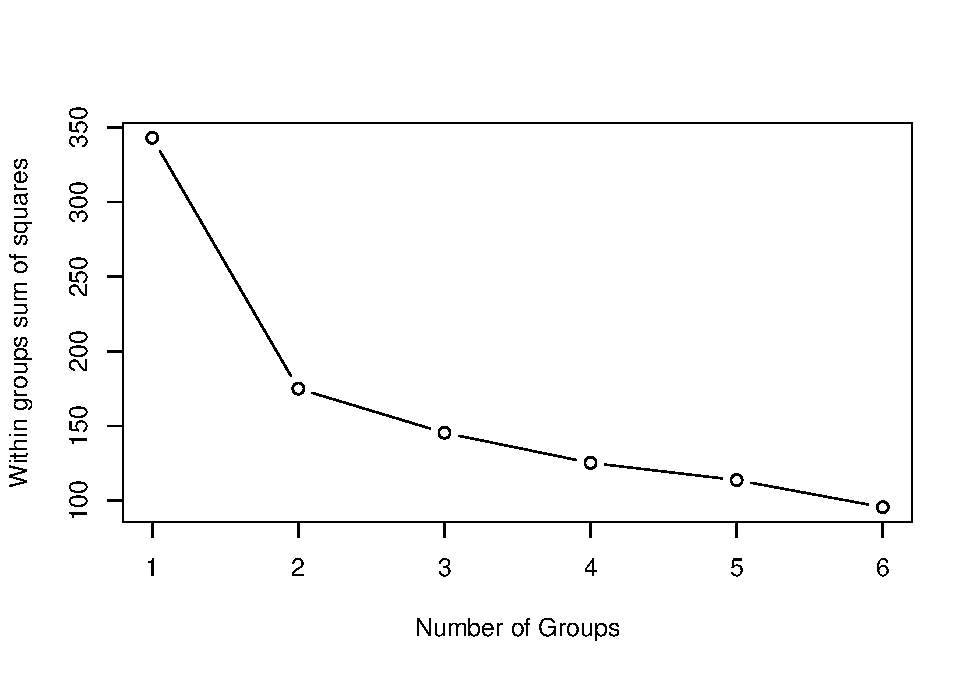
\includegraphics[width=0.5\linewidth,height=0.5\textheight]{HUDM6122-Homework_06-Chenguang-Pan_files/figure-latex/unnamed-chunk-1-1}

From the plot of within-group sum of squares for one- to six-cluster
solutions is similar to the textbook's result. The elbow occurs at the
two-group solution. Thus, I run the k-means method for this solutions.

\begin{Shaded}
\begin{Highlighting}[]
\SpecialCharTok{\textgreater{}} \FunctionTok{kmeans}\NormalTok{(df\_s, }\AttributeTok{centers=}\DecValTok{2}\NormalTok{)}
\NormalTok{K}\SpecialCharTok{{-}}\NormalTok{means clustering with }\DecValTok{2}\NormalTok{ clusters of sizes }\DecValTok{22}\NormalTok{, }\DecValTok{28}

\NormalTok{Cluster means}\SpecialCharTok{:}
\NormalTok{    Murder     Rape   Robbery  Assault Burglary    Theft  Vehicle}
\DecValTok{1} \FloatTok{2.711724} \FloatTok{3.132781} \FloatTok{2.1001609} \FloatTok{2.836238} \FloatTok{3.680055} \FloatTok{4.479685} \FloatTok{2.642471}
\DecValTok{2} \FloatTok{1.371839} \FloatTok{1.712574} \FloatTok{0.6770169} \FloatTok{1.308089} \FloatTok{2.203667} \FloatTok{3.411210} \FloatTok{1.177732}

\NormalTok{Clustering vector}\SpecialCharTok{:}
\NormalTok{ME NH VT MA RI CT NY NJ PA OH IN IL MI WI MN IA MO ND SD NE KS DE MD VA WV NC }
 \DecValTok{2}  \DecValTok{2}  \DecValTok{2}  \DecValTok{1}  \DecValTok{2}  \DecValTok{2}  \DecValTok{1}  \DecValTok{1}  \DecValTok{2}  \DecValTok{2}  \DecValTok{2}  \DecValTok{1}  \DecValTok{1}  \DecValTok{2}  \DecValTok{2}  \DecValTok{2}  \DecValTok{1}  \DecValTok{2}  \DecValTok{2}  \DecValTok{2}  \DecValTok{2}  \DecValTok{2}  \DecValTok{1}  \DecValTok{2}  \DecValTok{2}  \DecValTok{2} 
\NormalTok{SC GA FL KY TN AL MS AR LA OK TX MT ID WY CO NM AZ UT NV WA OR CA AK HI }
 \DecValTok{1}  \DecValTok{1}  \DecValTok{1}  \DecValTok{2}  \DecValTok{1}  \DecValTok{2}  \DecValTok{2}  \DecValTok{2}  \DecValTok{1}  \DecValTok{1}  \DecValTok{1}  \DecValTok{2}  \DecValTok{2}  \DecValTok{2}  \DecValTok{1}  \DecValTok{1}  \DecValTok{1}  \DecValTok{2}  \DecValTok{1}  \DecValTok{1}  \DecValTok{1}  \DecValTok{1}  \DecValTok{1}  \DecValTok{2} 

\NormalTok{Within cluster sum of squares by cluster}\SpecialCharTok{:}
\NormalTok{[}\DecValTok{1}\NormalTok{] }\FloatTok{102.3351}  \FloatTok{72.6241}
\NormalTok{ (between\_SS }\SpecialCharTok{/} \AttributeTok{total\_SS =}  \FloatTok{49.0}\NormalTok{ \%)}

\NormalTok{Available components}\SpecialCharTok{:}

\NormalTok{[}\DecValTok{1}\NormalTok{] }\StringTok{"cluster"}      \StringTok{"centers"}      \StringTok{"totss"}        \StringTok{"withinss"}     \StringTok{"tot.withinss"}
\NormalTok{[}\DecValTok{6}\NormalTok{] }\StringTok{"betweenss"}    \StringTok{"size"}         \StringTok{"iter"}         \StringTok{"ifault"}      
\end{Highlighting}
\end{Shaded}

Next, to visualize the result, I plot the two-group solution in the
space of the first two principal components of the correlation matrix of
the data.

\begin{Shaded}
\begin{Highlighting}[]
\SpecialCharTok{\textgreater{}}\NormalTok{ crime\_pca }\OtherTok{\textless{}{-}} \FunctionTok{prcomp}\NormalTok{(df\_s)}
\SpecialCharTok{\textgreater{}} \FunctionTok{plot}\NormalTok{(crime\_pca}\SpecialCharTok{$}\NormalTok{x[,}\DecValTok{1}\SpecialCharTok{:}\DecValTok{2}\NormalTok{],}
\SpecialCharTok{+}      \AttributeTok{pch =} \FunctionTok{kmeans}\NormalTok{(df\_s, }\AttributeTok{centers =} \DecValTok{2}\NormalTok{)}\SpecialCharTok{$}\NormalTok{cluster)}
\end{Highlighting}
\end{Shaded}

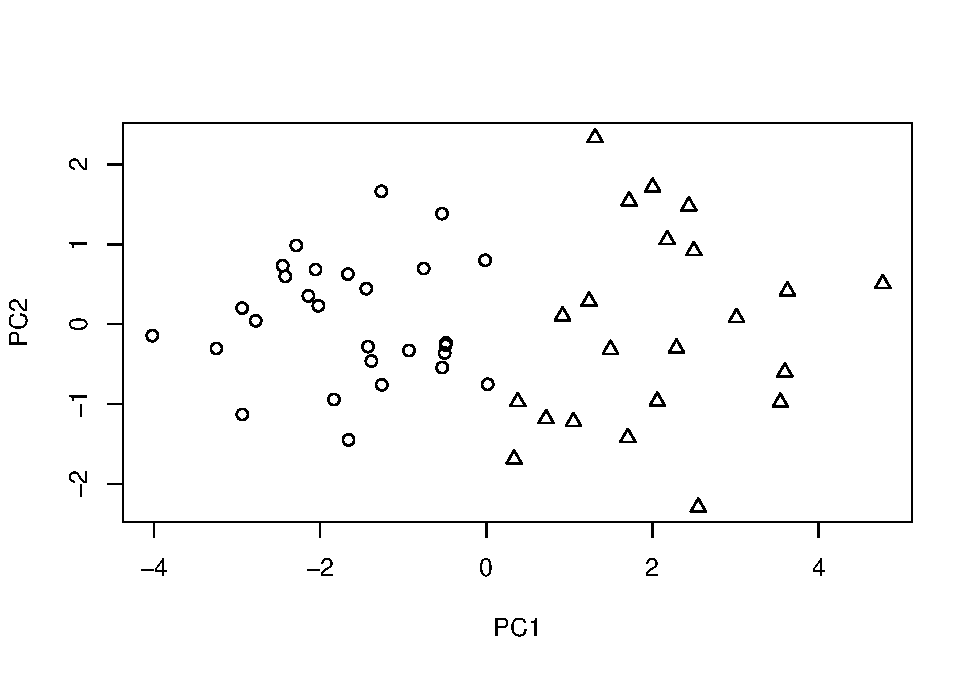
\includegraphics[width=0.5\linewidth,height=0.5\textheight]{HUDM6122-Homework_06-Chenguang-Pan_files/figure-latex/unnamed-chunk-3-1}

The result is similar to the plot found in the textbook. It suggests
that the cluster analysis here is dividing into two parts a homogeneous
set of data.

\hypertarget{ex-6.2}{%
\subsection{Ex 6.2}\label{ex-6.2}}

\emph{Calculate the first five principal components scores for the
Romano- British pottery data, and then construct the scatterplot matrix
of the scores, displaying the contours of the estimated bivariate
density for each panel of the plot and a boxplot of each score in the
appropriate place on the diagonal. Label the points in the scatterplot
matrix with their kiln numbers.}

\textbf{MY SOLUTION:}

Since the chemical elements are different scales, it is necessary to
standarize them first.

\begin{Shaded}
\begin{Highlighting}[]
\SpecialCharTok{\textgreater{}} \CommentTok{\# import the data}
\ErrorTok{\textgreater{}} \FunctionTok{data}\NormalTok{(}\StringTok{"pottery"}\NormalTok{, }\AttributeTok{package =} \StringTok{"HSAUR2"}\NormalTok{)}
\SpecialCharTok{\textgreater{}} \FunctionTok{dim}\NormalTok{(pottery)}
\NormalTok{[}\DecValTok{1}\NormalTok{] }\DecValTok{45} \DecValTok{10}
\SpecialCharTok{\textgreater{}} \CommentTok{\# run PCA for five{-}components solution; }
\ErrorTok{\textgreater{}} \CommentTok{\# since the chemical elements are at different scales, standardization is necessary.}
\ErrorTok{\textgreater{}} 
\ErrorTok{\textgreater{}}\NormalTok{ pca }\OtherTok{\textless{}{-}} \FunctionTok{prcomp}\NormalTok{(pottery[,}\SpecialCharTok{{-}}\DecValTok{10}\NormalTok{],}\AttributeTok{center =} \ConstantTok{TRUE}\NormalTok{)}
\SpecialCharTok{\textgreater{}}\NormalTok{ scores }\OtherTok{\textless{}{-}}\NormalTok{ pca}\SpecialCharTok{$}\NormalTok{x[,}\DecValTok{1}\SpecialCharTok{:}\DecValTok{5}\NormalTok{]}
\end{Highlighting}
\end{Shaded}

Next, I use the scores of the first five principal components scores to
construct the scatterplot matrix of the scores.

\begin{Shaded}
\begin{Highlighting}[]
\SpecialCharTok{\textgreater{}} \CommentTok{\# create a scatterplot matrix with density contours}
\ErrorTok{\textgreater{}} \FunctionTok{pairs}\NormalTok{(scores, }
\SpecialCharTok{+}       \AttributeTok{main =} \StringTok{"Scatterplot Matrix of Pottery Data Principal Component Scores"}\NormalTok{,}
\SpecialCharTok{+}       \AttributeTok{upper.panel =} \ControlFlowTok{function}\NormalTok{(x, y) \{}
\SpecialCharTok{+}         \FunctionTok{points}\NormalTok{(x, y)}
\SpecialCharTok{+}\NormalTok{         den }\OtherTok{\textless{}{-}}\NormalTok{ MASS}\SpecialCharTok{::}\FunctionTok{kde2d}\NormalTok{(x,y)}
\SpecialCharTok{+}         \FunctionTok{contour}\NormalTok{(den, }\AttributeTok{add =} \ConstantTok{TRUE}\NormalTok{,}\AttributeTok{col=}\StringTok{"red"}\NormalTok{,}\AttributeTok{lwd=}\DecValTok{1}\NormalTok{)}
\SpecialCharTok{+}\NormalTok{       \},}
\SpecialCharTok{+}       \AttributeTok{diag.panel =} \ControlFlowTok{function}\NormalTok{(x) \{}
\SpecialCharTok{+}         \FunctionTok{boxplot}\NormalTok{(x, }\AttributeTok{horizontal =}\NormalTok{ T, }\AttributeTok{add =} \ConstantTok{TRUE}\NormalTok{)}
\SpecialCharTok{+}\NormalTok{       \},}
\SpecialCharTok{+}       \AttributeTok{lower.panel =} \ControlFlowTok{function}\NormalTok{(x, y) \{}
\SpecialCharTok{+}         \FunctionTok{points}\NormalTok{(x, y)}
\SpecialCharTok{+}         \FunctionTok{text}\NormalTok{(x, y, pottery}\SpecialCharTok{$}\NormalTok{kiln, }\AttributeTok{pch =} \DecValTok{16}\NormalTok{, }\AttributeTok{col =} \FunctionTok{adjustcolor}\NormalTok{(}\StringTok{"blue"}\NormalTok{, .}\DecValTok{5}\NormalTok{))\})}
\SpecialCharTok{\textgreater{}} \CommentTok{\# Add kiln number labels to the scatterplot matrix}
\ErrorTok{\textgreater{}} \FunctionTok{text}\NormalTok{(scores, }\AttributeTok{labels =}\NormalTok{ pottery}\SpecialCharTok{$}\NormalTok{kiln, }\AttributeTok{pos =} \DecValTok{1}\NormalTok{, }\AttributeTok{cex =} \FloatTok{0.1}\NormalTok{)}
\end{Highlighting}
\end{Shaded}

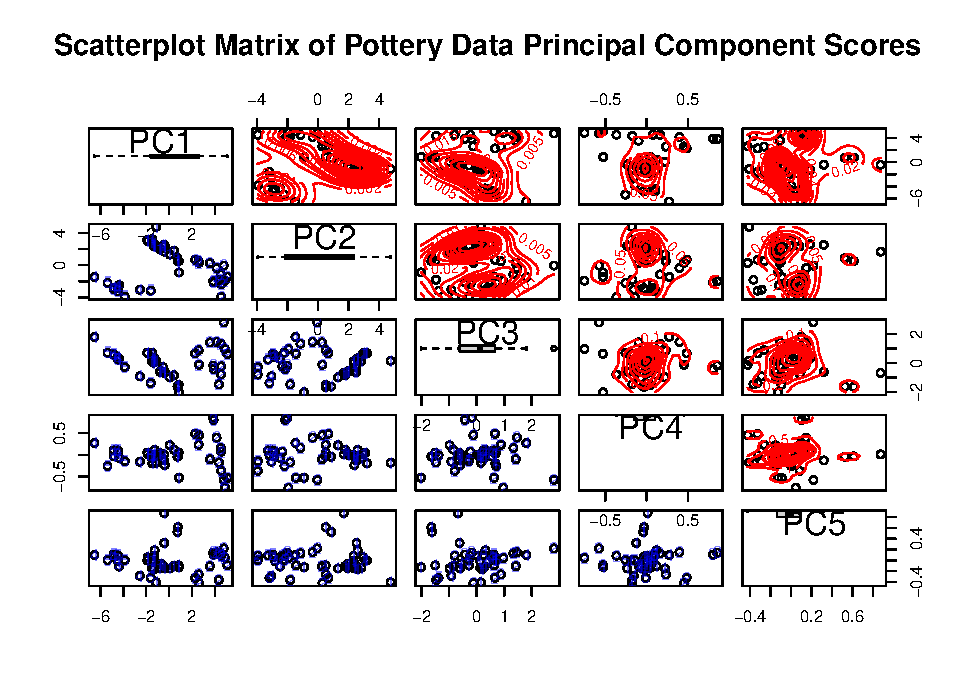
\includegraphics{HUDM6122-Homework_06-Chenguang-Pan_files/figure-latex/unnamed-chunk-5-1.pdf}

\hypertarget{ex-6.3}{%
\subsection{Ex 6.3}\label{ex-6.3}}

\emph{Return to the air pollution data given in Chapter 1 and use finite
mixtures to cluster the data on the basis of the six climate and ecology
variables (i.e., excluding the sulphur dioxide concentration).
Investigate how sulphur dioxide concentration varies in the clusters you
find both graphically and by formal significance testing.}

\textbf{MY SOLUTION:}\\
One thing that is quite tricky here is how to rely on BIC to choose the
best model. It seems to be conflicting to our normal understanding about
AIC and BIC. I'd like to write down some understanding here for my
future reference.

AIC and BIC are commonly used to compare the fit of different models,
and to select the best model among a set of candidate models. The basic
idea behind AIC and BIC is that they attempt to balance the
goodness-of-fit of the model with the complexity of the model. AIC and
BIC both penalize models that are too complex, but BIC applies a
stronger penalty for model complexity than AIC. The model with the
lowest AIC or BIC is generally considered the best model among the set
of candidate models.

However, in finite mixture approach, the larger the value of the BIC,
the stronger the evidence for the model and number of clusters. But why?
I did some literature review and did not find any clues. I will continue
to figure out this issue.

\begin{Shaded}
\begin{Highlighting}[]
\SpecialCharTok{\textgreater{}} \CommentTok{\# import the data}
\ErrorTok{\textgreater{}} \FunctionTok{data}\NormalTok{(}\StringTok{"USairpollution"}\NormalTok{, }\AttributeTok{package =} \StringTok{"HSAUR2"}\NormalTok{)}
\SpecialCharTok{\textgreater{}} \FunctionTok{dim}\NormalTok{(USairpollution)}
\NormalTok{[}\DecValTok{1}\NormalTok{] }\DecValTok{41}  \DecValTok{7}
\SpecialCharTok{\textgreater{}} \FunctionTok{colnames}\NormalTok{(USairpollution)}
\NormalTok{[}\DecValTok{1}\NormalTok{] }\StringTok{"SO2"}     \StringTok{"temp"}    \StringTok{"manu"}    \StringTok{"popul"}   \StringTok{"wind"}    \StringTok{"precip"}  \StringTok{"predays"}
\SpecialCharTok{\textgreater{}} 
\ErrorTok{\textgreater{}} \CommentTok{\# before running the finite mixture approach, standardize the data first;}
\ErrorTok{\textgreater{}} \CommentTok{\# air\_sdz \textless{}{-} sweep(USairpollution,2,apply(USairpollution[,{-}1], 2, sd), FUN = "/")}
\ErrorTok{\textgreater{}}\NormalTok{ air\_s }\OtherTok{\textless{}{-}} \FunctionTok{scale}\NormalTok{(USairpollution)}
\SpecialCharTok{\textgreater{}} 
\ErrorTok{\textgreater{}} \CommentTok{\# run the finite mixtures to the cluster the data}
\ErrorTok{\textgreater{}} \CommentTok{\# install.packages("mclust")}
\ErrorTok{\textgreater{}} \FunctionTok{library}\NormalTok{(mclust)}
\SpecialCharTok{\textgreater{}}\NormalTok{ mc }\OtherTok{\textless{}{-}} \FunctionTok{Mclust}\NormalTok{(air\_s[,}\SpecialCharTok{{-}}\DecValTok{1}\NormalTok{])}
\SpecialCharTok{\textgreater{}} \FunctionTok{plot}\NormalTok{(mc}\SpecialCharTok{$}\NormalTok{BIC)}
\end{Highlighting}
\end{Shaded}

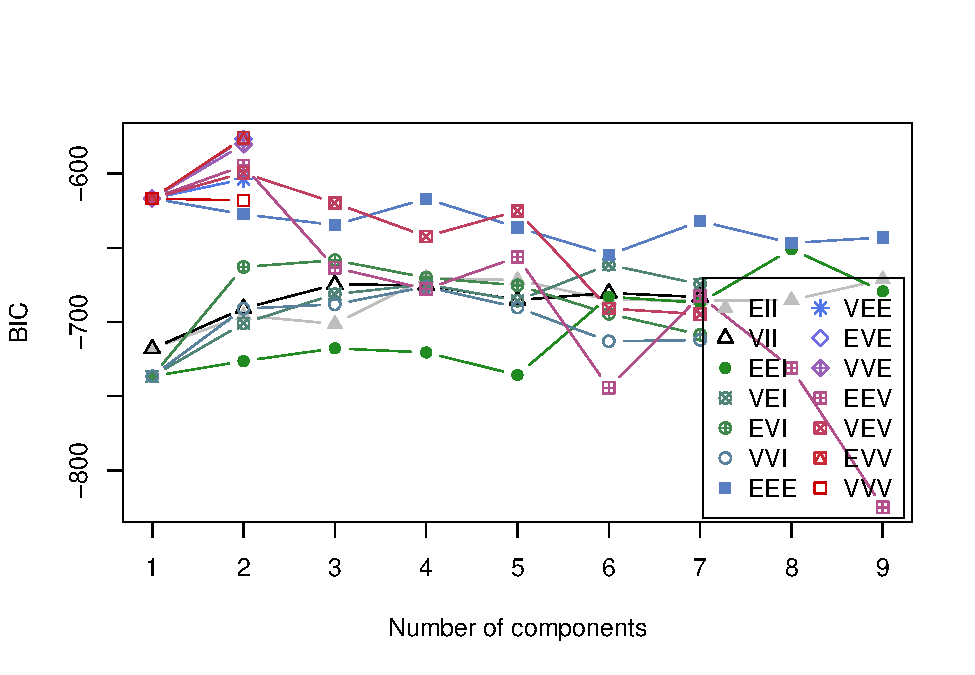
\includegraphics{HUDM6122-Homework_06-Chenguang-Pan_files/figure-latex/unnamed-chunk-6-1.pdf}
The BIC criterion selects model EVV and two clusters as the optimal
solution.

\begin{Shaded}
\begin{Highlighting}[]
\SpecialCharTok{\textgreater{}} \CommentTok{\# For the following method, I refereed to Xue Yu\textquotesingle{}s idea. Thanks for her help.}
\ErrorTok{\textgreater{}} \FunctionTok{boxplot}\NormalTok{(USairpollution}\SpecialCharTok{$}\NormalTok{SO2}\SpecialCharTok{\textasciitilde{}}\NormalTok{ mc}\SpecialCharTok{$}\NormalTok{classification)}
\end{Highlighting}
\end{Shaded}

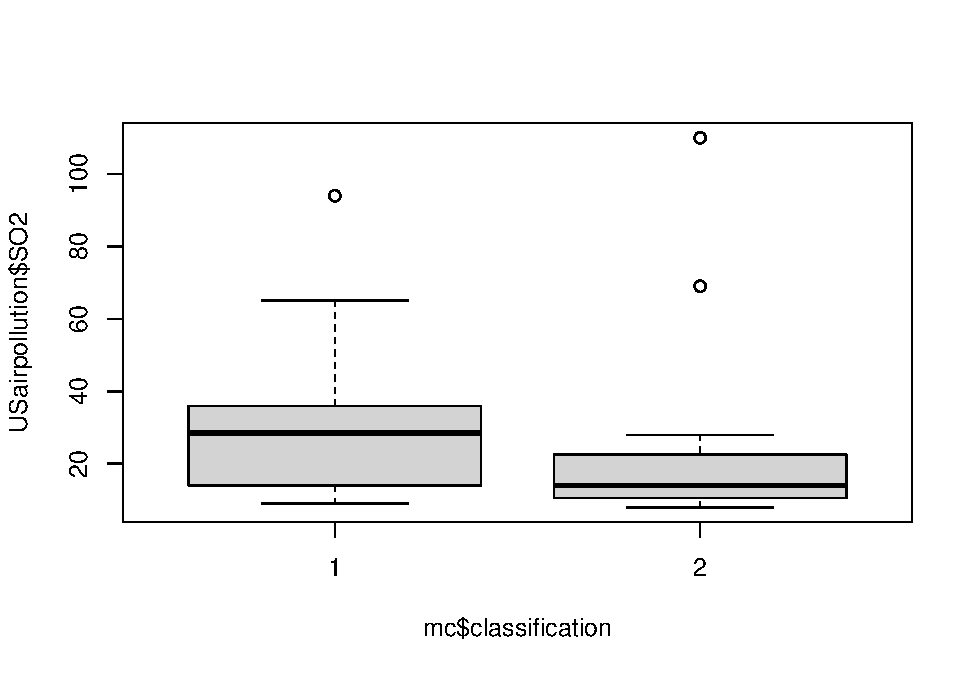
\includegraphics{HUDM6122-Homework_06-Chenguang-Pan_files/figure-latex/unnamed-chunk-7-1.pdf}
The boxplot shows that there seems no significant difference between the
two clusters in SO2 concentration. Next, I will run a two sample t test
to figure out the relation.

\begin{Shaded}
\begin{Highlighting}[]
\SpecialCharTok{\textgreater{}} \FunctionTok{t.test}\NormalTok{(USairpollution}\SpecialCharTok{$}\NormalTok{SO2}\SpecialCharTok{\textasciitilde{}}\NormalTok{mc}\SpecialCharTok{$}\NormalTok{classification)}

\NormalTok{    Welch Two Sample t}\SpecialCharTok{{-}}\NormalTok{test}

\NormalTok{data}\SpecialCharTok{:}\NormalTok{  USairpollution}\SpecialCharTok{$}\NormalTok{SO2 by mc}\SpecialCharTok{$}\NormalTok{classification}
\NormalTok{t }\OtherTok{=} \FloatTok{0.30473}\NormalTok{, df }\OtherTok{=} \FloatTok{12.88}\NormalTok{, p}\SpecialCharTok{{-}}\NormalTok{value }\OtherTok{=} \FloatTok{0.7654}
\NormalTok{alternative hypothesis}\SpecialCharTok{:}\NormalTok{ true difference }\ControlFlowTok{in}\NormalTok{ means between group }\DecValTok{1}\NormalTok{ and group }\DecValTok{2}\NormalTok{ is not equal to }\DecValTok{0}
\DecValTok{95}\NormalTok{ percent confidence interval}\SpecialCharTok{:}
 \SpecialCharTok{{-}}\FloatTok{19.34158}  \FloatTok{25.68703}
\NormalTok{sample estimates}\SpecialCharTok{:}
\NormalTok{mean }\ControlFlowTok{in}\NormalTok{ group }\DecValTok{1}\NormalTok{ mean }\ControlFlowTok{in}\NormalTok{ group }\DecValTok{2} 
       \FloatTok{30.90000}        \FloatTok{27.72727} 
\end{Highlighting}
\end{Shaded}

The test result also indicates that there is no significant difference
in SO2 concentration in the two clusters, \emph{t}= .305, \emph{p}
=.765.

\end{document}
